\section{Introduction}
\label{sec:intro}

Query Segmentation is an important task in Information Retrieval (IR).
A query is a sequence of words (in English) or characters (in Chinese) which carries the information requirement of a user.
Query segmentation task is to cut a query into several continuous subsequences called \emph{segments} which are normally frequently-used phases.
These meaningful segments instead of independent words or characters in the query are significant to the search engine.
Assuming a user looking for ``short sleeve long dress'', ``short sleeve'' and ``long dress'' are two segments which indicate a long dress with short sleeve.
If the query is processed based on independent words, many needless short dresses with long sleeve may be returned. 
The quality of query segmentation is very important to the downstream IR task.

With the rapid development of online e-commerce platforms such as Amazon (in English) and Taobao (in Chinese),
query segmentation in e-commerce field should receive more attention.
Here we focus on e-commerce query segmentation in Chinese.
In e-commerce field, queries are used to describe some kind of product.
The segments of these queries are usually brand names, product names, attribute names or attribute values.
For example, a query ``高腰连衣裙白色 (high-waisted dress white)'' consists of $3$ segments ``高腰 (high-waisted) / 连衣裙 (dress) / 白色 (white)''.
The segment ``dress'' is a product name, ``high-waisted'' and ``white'' are attribute values used to provide details of product ``dress''.

Query segmentation task has been studied extensively in research community.
Most of methods can be divided into three categories: unsupervised \cite{risvik_query_2003,zhang_query_2009,kiseleva_unsupervised_2010,mishra_unsupervised_2011,parikh_segmentation_2013,hagen_power_2010,hagen_query_2011,tan_unsupervised_2008,huang_exploring_2010},
feature-based supervised \cite{yu_query_2009,du_perceptron-based_2014}
and deep learning methods \cite{kale_towards_2017,lin_query_2017}.
Unsupervised methods score each segmentation combination of a query by some kinds of statistical indexes like mutual information \cite{risvik_query_2003}.
Feature-based and deep learning methods are supervised, and rely on a large number of gold segmented queries.
Supervised methods especially deep learning are attractive for better performance and are focused in our work,
but lack of labeled data is one of big challenges for training deep neural networks.
In this work we borrow the idea of long-distance supervision \cite{mintz2009distant} to automatically create large amounts of gold standard data.
In e-commerce field,
because queries are related to products,
we build a dictionary by crawling brand names, product names, attribute names and attribute values from the product detail pages of online shopping platforms.
Then a simple max-matching algorithm can be used to segment queries by matching subsequences in queries with the words in dictionary.

Another challenge of query segmentation task is Out-of-Vocabulary (OOV) segments.
OOV segments are those segments which are used in test queries but do not appear in training queries.
OOV issue has been studied widely in Chinese Word Segmentation (CWS) task
\cite{Xue2003Chinese,Jin2005A,Zhao2006An,huang2007chinese,Zheng2013Deep} which is a very similar task with query segmentation.
\cite{huang2007chinese} argues that OOV is the key problem of CWS task.
We argue that OOV also impacts the performance of query segmentation to a large extent.
We try to alleviate OOV issue by incorporating contexts from external documents.
If the OOV segments can be found in external documents, we can extract some valuable features to help to recognize those.

We treat query segmentation as a sequence labeling problem.
The tagging scheme consists of ``B'' and ``I''.
``B'' (Begin) means current character is the head of its segment,
while ``I'' (Inner) means current character belongs to previous segment.
%For example, in Fig. \ref{fig:sq}, ``dress'' is a segment of query ``高腰连衣裙白色''.
%Because ``连'' is the begin of this segment, its label is ``B''.
%And the labels of ``衣'' and ``裙'' are ``I'' and ``I''.
An example is shown in Figure \ref{fig:sq}.
\begin{figure}[th]
	\centering
	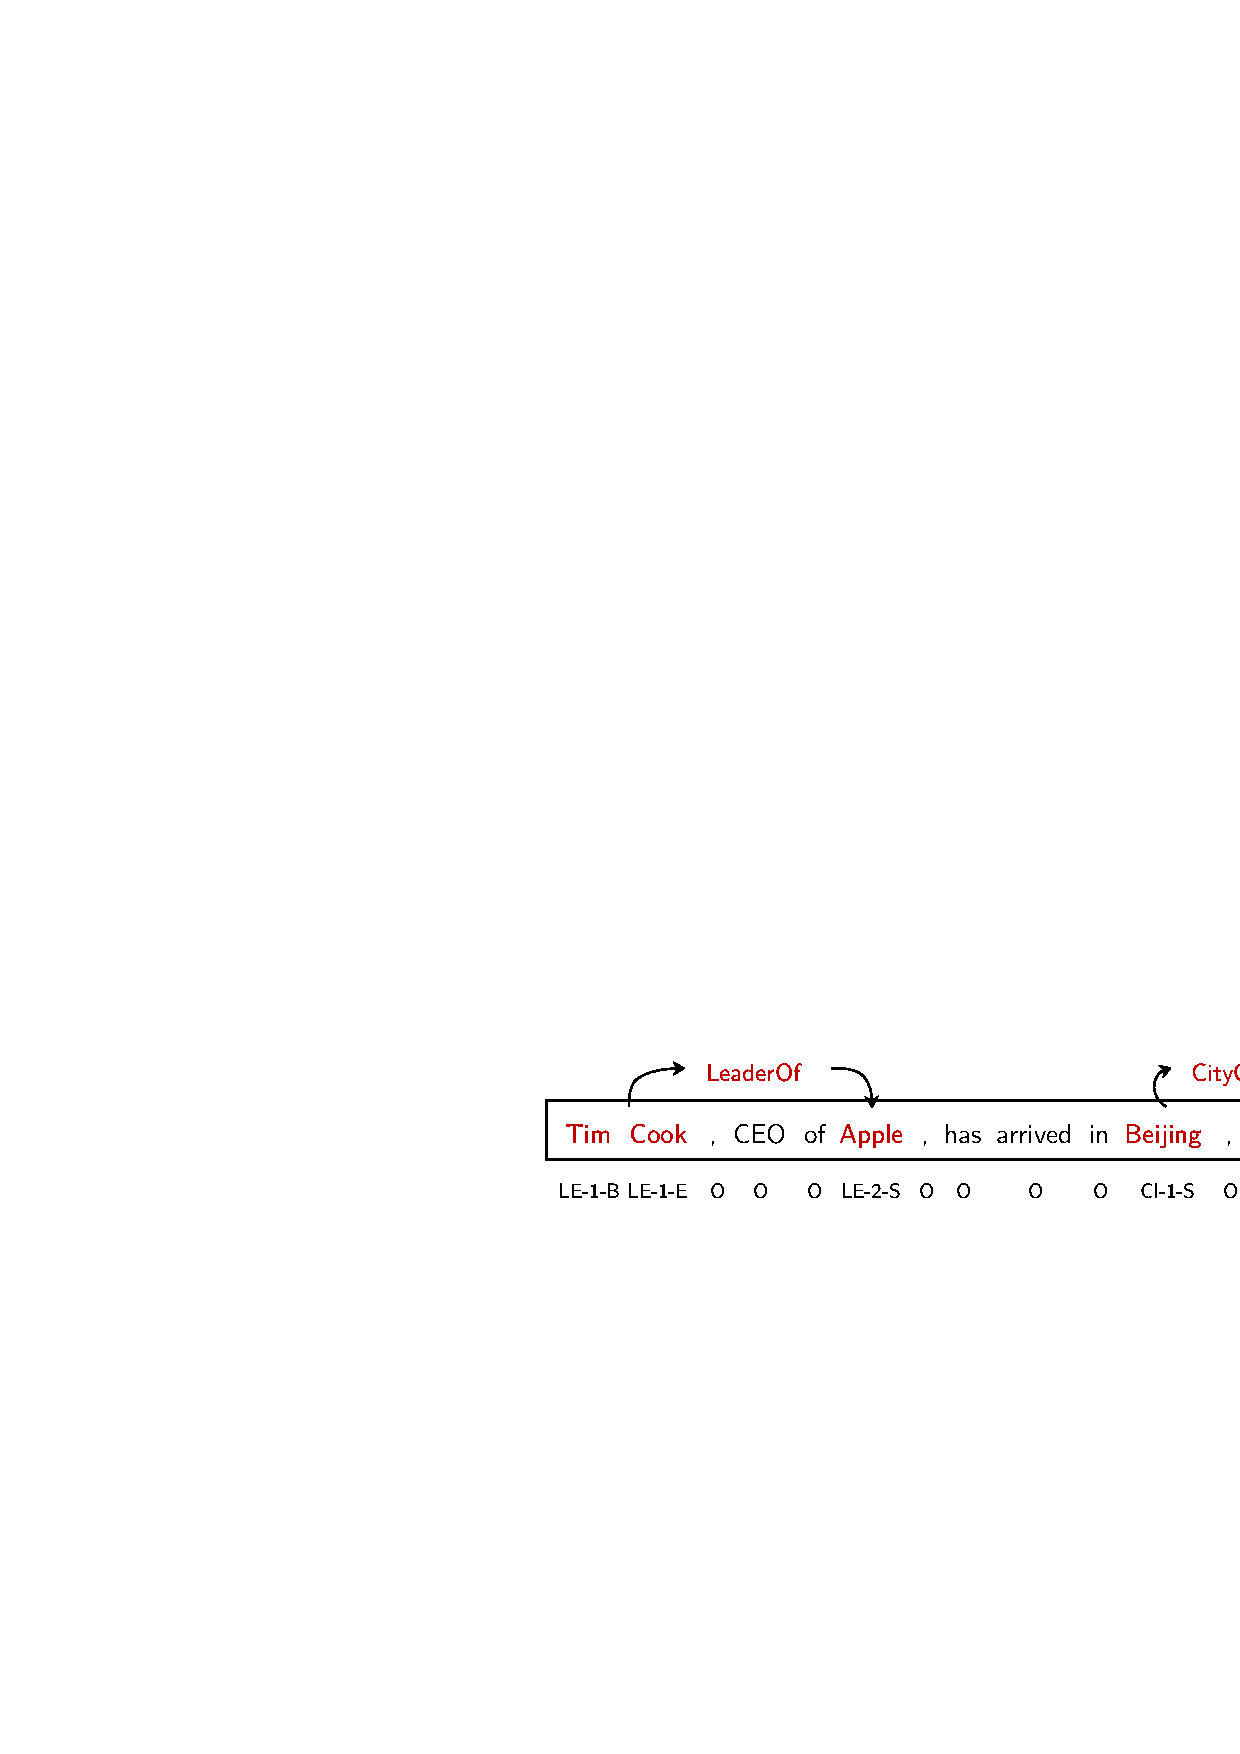
\includegraphics[width=0.45\columnwidth]{figures/introduction.pdf}
	\caption{The segmentation result is ``高腰 (high-waisted) / 连衣裙 (dress) / 白色 (white)''. Therefore, the label sequence of this query is ``B/I/B/I/I/B/I''.}
	\label{fig:sq}
\end{figure}
Under this tagging scheme,
the target is to predict one label of ``B'' and ``I'' for each character in a query.
Our approach contains two step.
First step is to find contexts for each character in queries and extract features from these contexts.
Second step is to train our neural networks model using these extracted features.
As for each character in queries, we can get its left and right bi-grams. For example, the left and right bi-grams of character ``衣'' in query ``高腰连衣裙白色'' are ``连衣'' and ``衣裙''. 
We search these two bi-grams in external documents.
All sentences which contain any one of them are treated as contexts of this character.
All the contexts of a character is called context bag.
For each context in context bag, we use same method to extract features and get the feature bag.
BiLSTM-CRF \cite{Huang2015Bidirectional,Ma2016End} is a common model to deal with sequence labeling problem.
It can be used to our query segmentation directly.
To utilize the feature bag from external documents,
we design our model by improving the normal BiLSTM-CRF model,
we use attention mechanism \cite{bahdanau2014neural} to encode the feature bag and get its vector representation.
Then we add this vector representation of feature bag to the common BiLSTM-CRF.
The helpful information contained in contexts will help to predict labels.

% Because of contexts from external documents, we argue that our approach can alleviate the OOV problem to large extent. For OOV words which do not appear in training queries, if the external documents share a relavent topic with these queries, it is possible to find these OOV words in the documents. In other words, we can still find contexts for these OOV words, which can provide features to recognize the boundaries of them. Also for words already in training queries, the found contexts can still provide valuable features and be helpful for predicting their labels.


Our main contributions are as follows:
\begin{itemize}
	\item We borrow the idea of distant supervision method and propose a effective method to label e-commerce queries automatically, which address the lack of labeled data.
	\item We design to improve the common BiLSTM-CRF model by including attention to contexts information from external documents, which can alleviate the issue of OOV.
	\item Experiments on two e-commerce datasets shows that our model can achieve 0.049 and 0.023 improvements in F1 value above the strongest baselines.
\end{itemize}


